\graphicspath{{images/}}

\section{Results}
\label{sec:results}

% \subsection{\thesubsection~Guessing}
% \end{multicols}
% \graphicspath{{images/guessing/}}
% \begin{Figure}
%   \centering
%   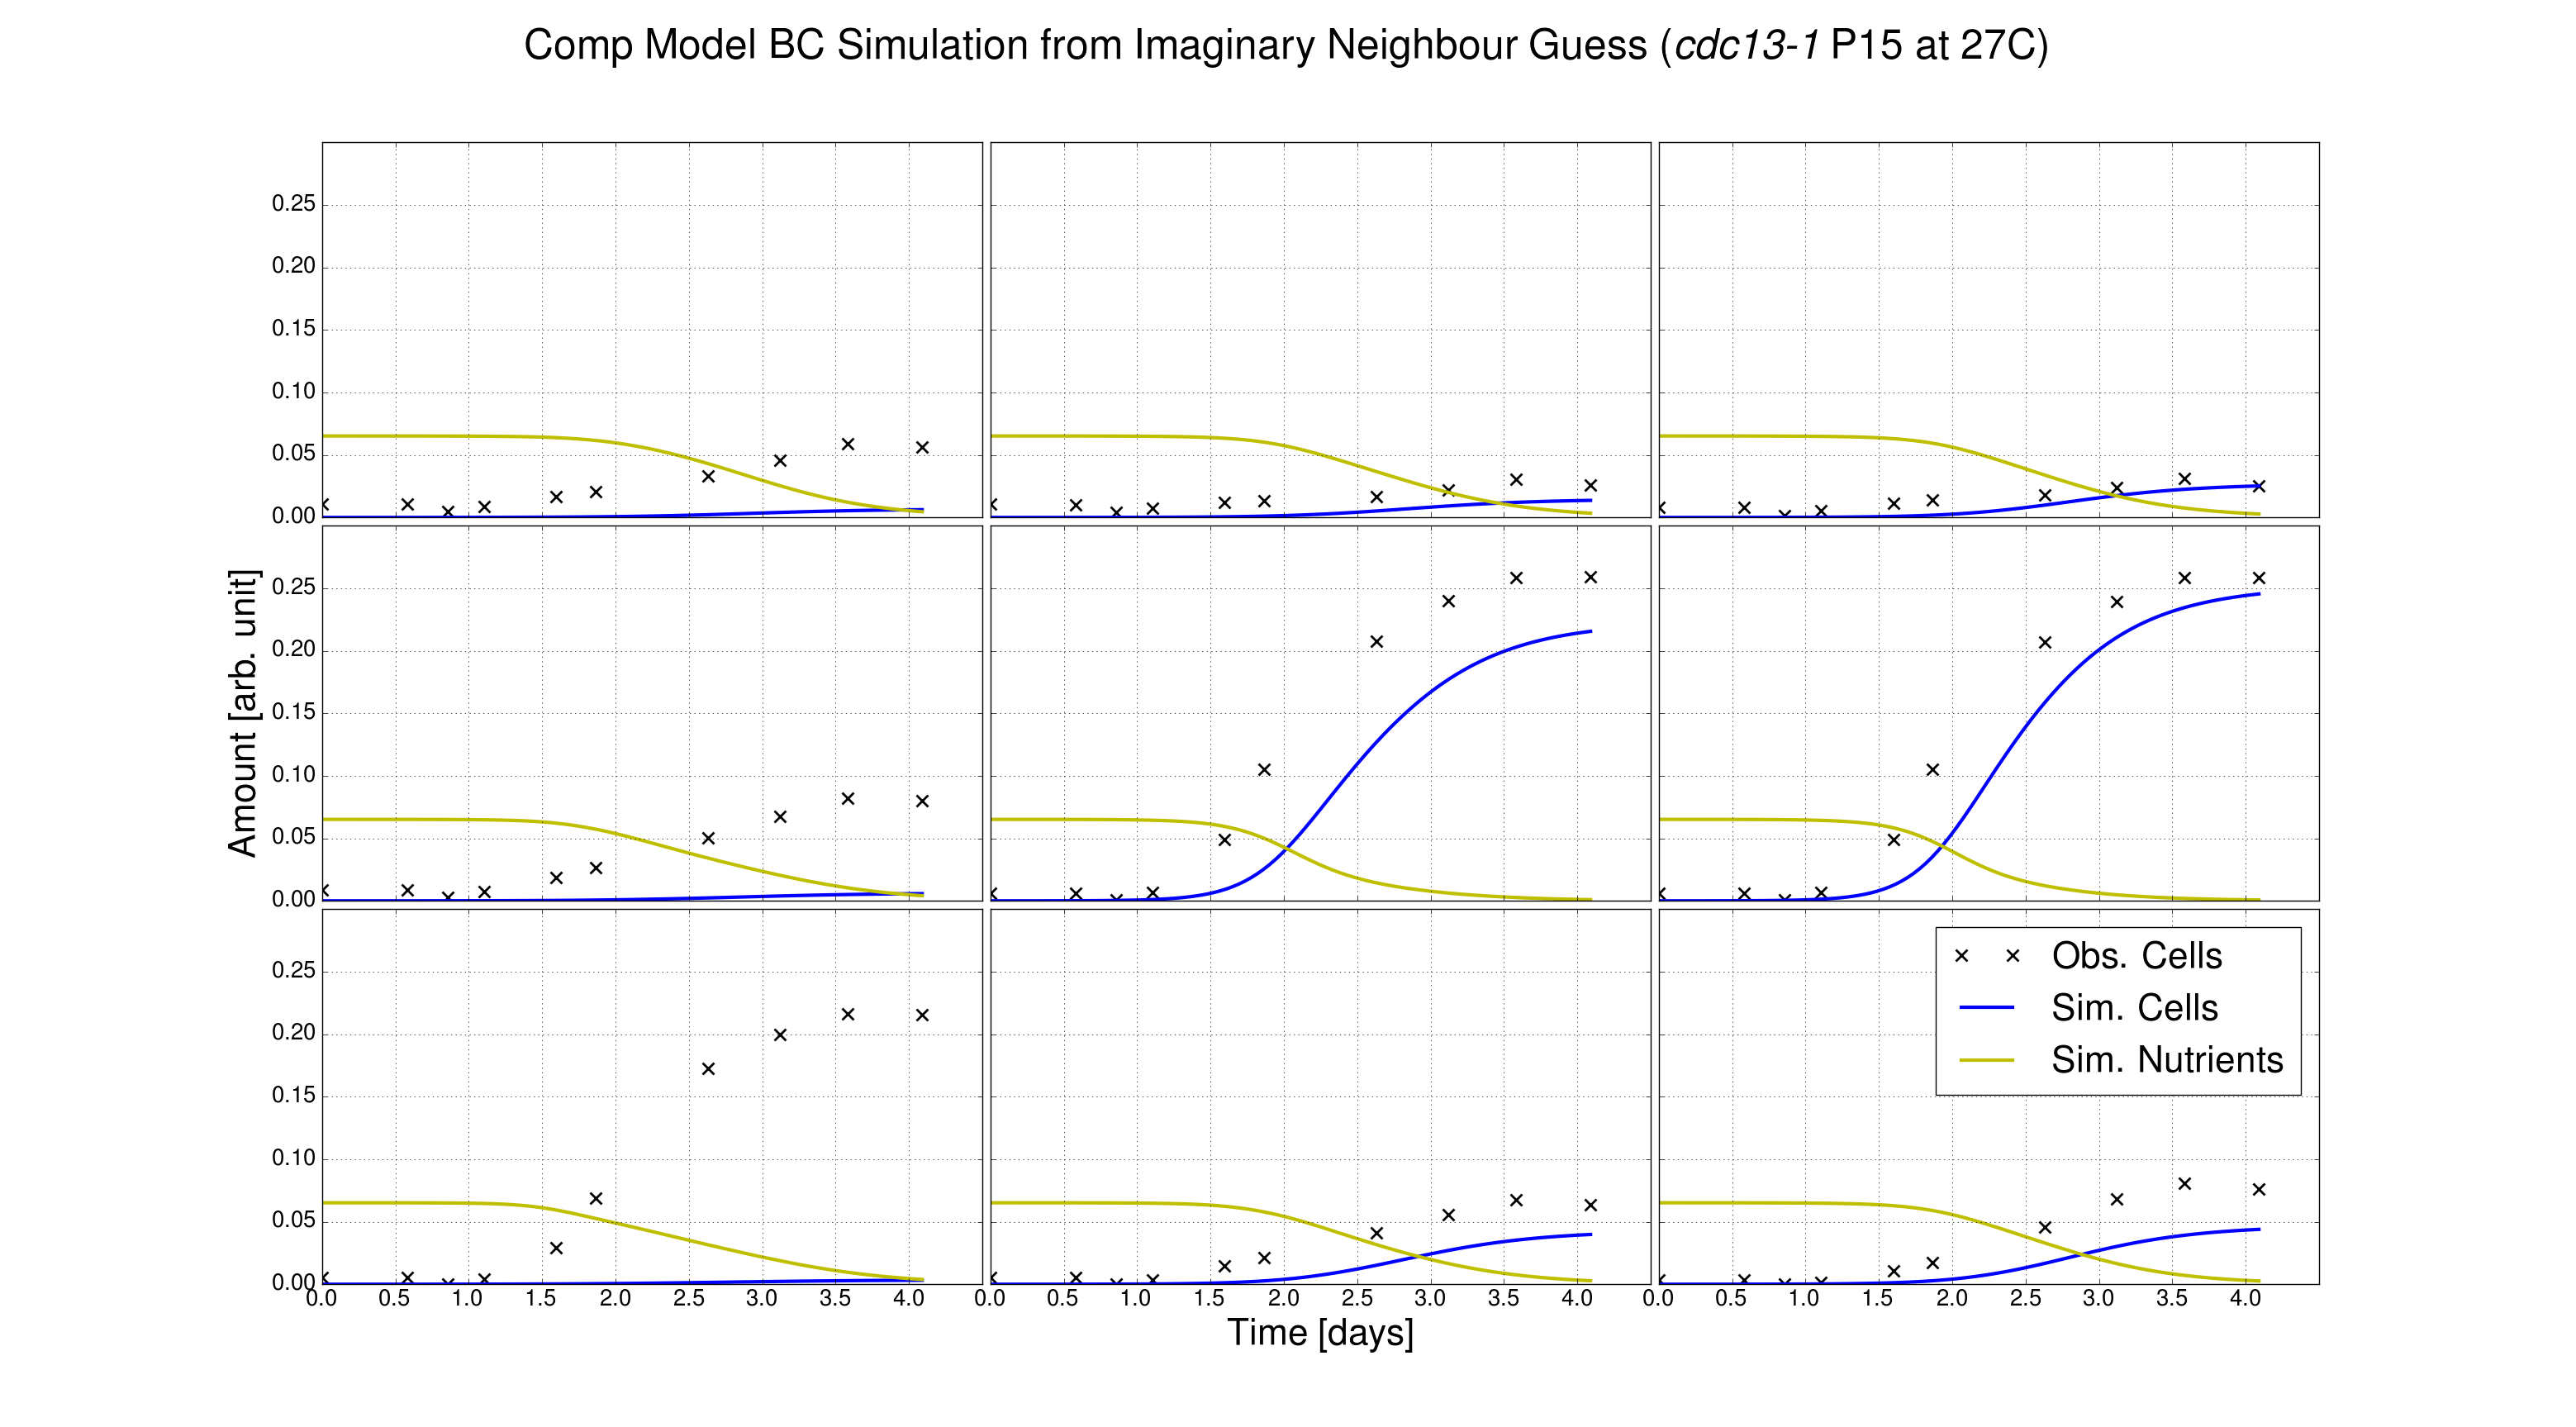
\includegraphics[width=\linewidth]{final/P15_R5_C18_guess_sim}
%   \captionof{figure}{\textbf{Competition model simulation using
%       parameters from imaginary neighbour guessing.} Shows a 3x3 zone
%     with top-left coordinate (5, 18) from P15 with background
%     \textit{cdc13-1} at 27\(^{\circ}C\).}
%   \label{fig:imag_neigh_guess_sim}
% \end{Figure}
% \begin{multicols}{2}

% Scripts were run with combinations of the following values.
% cellratios = np.logspace(-3, -5, num=5)
% fittype = ["imagneigh", "logeq"]
% zerokn = [True, False]

% Each script looped through the following array of b values which were
% supplied to the initial guesser and used at the plate level.

% for b-guess in [35, 40, 45, 50, 55, 60, 65, 70, 75, 80, 95, 100, 150]:

\subsection{Model comparison using P15}
\label{sec:P15_fit}
\subsubsection{Quality of fit}

I compared the competition and logistic models by fitting both to P15
(data described in Section~\ref{sec:P15_description}). For the
competition model, I used five values of \(C(0)\) over the range
\(N(0)\times\)10\(^{-5} < C(0) < N(0)\times\)10\(^{-3}\) to make
initial parameter guesses as described in
Section~\ref{sec:initial_guess}. This generated 70 initial parameter
sets which I used in 70 separate fits. Cell density estimates fit data
closely Figure~\ref{fig:comp_fit_plate}.
% Timecourses for the best fit are shown in
% Figure~\ref{fig:comp_fit_plate}. Cell density estimates fit data
% closely.
A high nutrient diffusion constant, \(k\), is estimated, such that
nutrients diffuse readily and nutrient timecourses are similar across
local areas of the plate. Estimated parameters for the two closest
fits are show in Table~\ref{tab:P15_best_fit_params}. \(N_{I}(0)\) and
\(N_{E}(0)\) agree better than \(C(0)\) and \(k\). It appears that the
gradient method is not finding a global minimum. However, \(b_{i}\)
estimates are correlated with Spearman's rank correlation coefficient,
\(\rho_{S} = 0.989\), and have average mean absolute deviation,
\(MAD = 1.56\). The mean value of \(b\) for the best fit is 44.4, so
agreement between \(b_{i}\) are good. This is important because \(b\)
is to be used as a fitness estimate to compare with the logistic
model.
\begin{center}
  \captionof{table}{\textbf{Estimated parameters for the two best
      competition model fits to P15.} Spearman's rank correlation
    coefficient (\(\rho_{S}\)) between \(b\) estimates is 0.989. Mean
    absolute deviation (MAD) between \(b\) estimates is 1.56. Obj.~is
    the total objective function value for internal cultures (smaller
    values are better).}
  \begin{tabular}{l l l l l l}
    \hline
    Fit     & \(C(0)\)                    & \(N_{I}(0)\) & \(N_{E}(0)\) & \(k\) & Obj.\\
    \hline
    1st     & 9.1\(\times\)10\(^{-5}\)    & 0.064      & 0.090       & 6.7  & 0.194 \\
    2nd     & 13.9\(\times\)10\(^{-5}\)   & 0.062      & 0.097       & 8.3  & 0.196 \\
    \hline
  \end{tabular}
  \label{tab:P15_best_fit_params}
\end{center}

% For all comparisons between the top four fits, \(\rho_{S}\) ranges
% from 0.922 to 0.995 and \(b\) MAD ranges from 1.56 to 6.90. I
% discarded the 5th best fit, which has less agreement, because, unlike
% the other fits, it estimated \(N_{I}(0)\) > \(N_{E}(0)\). When
% comparing this outlier with the top four fits, \(\rho_{S}\) is above
% 0.930, but \(b_{i}\) are more affected, with a maximum MAD of
% 13.29. Despite not finding a global minimum, the best competition
% model estimates of \(b_{i}\) agree well enough with each to allow
% meaningful comparison with logistic model parameter estimates.

The boxed 3x3 zone in Figure~\ref{fig:comp_fit_plate} is replotted in
Figure~\ref{fig:P15_zone_fit} with fits of the competition model
(solid blue and yellow), initial guess (dashed blue and yellow), and
logistic model (solid red). The zone contains more fast growing
cultures than is typical for the plate, so competition effects might
be greater than average.
% The logistic model was fit using the QFA R package \citep{qfa2016}.
The fit of the initial guess is typical for the plate: timecourses for
some cultures, such as the bottom-left, are poor. Nevertheless, the
guess fulfils its purpose by allowing a good fit of the competition
model to be made. Objective function values for the logistic and
competition model are similar for most cultures in the zone. For the
centre and centre-right fast growing cultures, however, the
competition model has much lower objective function values and fits
are closer. The total objective function value for the zone is lower
for the competition model: 44.06 vs 68.38 (values scaled by
\(10^{4}\)). This is not typical for the plate; objective function
values are on average slightly better for the logistic model (see
Table~\ref{tab:P15_obj_fun}). Recall that only internal objective
function values are used to assess the fit. Overall, the competition
model performed well considering that it used far fewer parameters
(387 vs 1152).


\graphicspath{{images/p15_fits/}}
\begin{Figure}
  \centering
  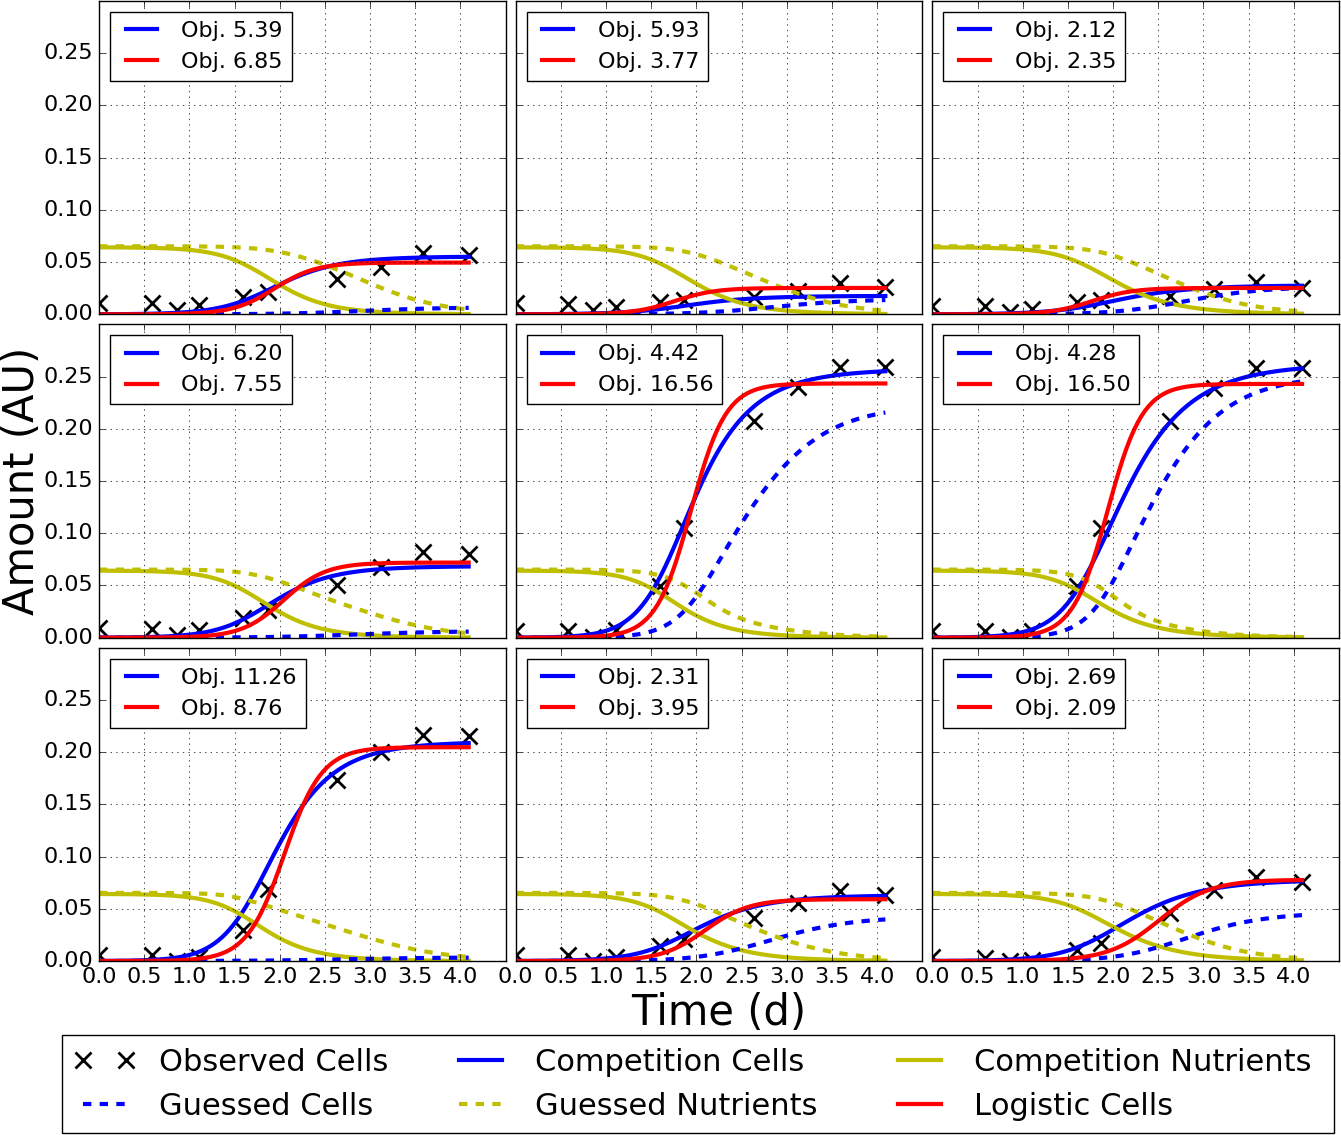
\includegraphics[width=\linewidth]{final/zone_r5_c18_with_obj_fun_2}
  \captionof{figure}{\textbf{A 3x3 zone of P15 showing fits of the
      competition and logistic models}. The zone has top-left
    coordinates (5, 18) and is boxed in red in
    Figure~\ref{fig:comp_fit_plate}. This is a zoom on a whole plate
    fit, not just a fit to the zone. Fits are for the competition
    model (blue and yellow solid); logistic model (solid red), and
    initial guess (blue and yellow dashed). Objective function values
    (Obj.), scaled by \(10^{4}\), are displayed for each culture
    (smaller values are better).}
  \label{fig:P15_zone_fit}
\end{Figure}
\begin{center}
  \captionof{table}{\textbf{Objective function values for competition
      and logistic model fits to P15.} ``Internal'' is the total
    objective function value for cultures not at an edge and is used
    to select the best fit. ``All'' is the total objective function
    value for all cultures on the plate. Smaller values are better.}
  \begin{tabular}{l l l}
    \hline
    Cultures     & Competition & Logistic \\
    \hline
    Internal     & 0.194    & 0.155\\
    All          & 0.465    & 0.345\\
    \hline
  \end{tabular}
  \label{tab:P15_obj_fun}
\end{center}

\subsubsection{\boldmath Correlation of fitness estimates \unboldmath}
\label{sec:correlation}

To compare fitness estimates between models, I converted competition
model \(b\) to logistic model \(r\) using (\ref{eq:conversion}).
% I took the median \(r\) for each deletion for both the competition
% and logistic model. I took the median, rather than mean, to reduce
% the effect of outliers that may results from cross-contamination of
% strains or inoculation of dead cells.
I plotted correlation between \(r\) estimates for each culture (black)
and between median \(r\) estimates for each deletion (red)
(Figure~\ref{fig:P15_correlations}).
% competiton model r is corrected to independent conditions.
For individual cultures, the competition model distribution is
unimodal, the logistic model distribution bimodal with minimum at
\(r \approx 4\). There are two distinct correlated groups: the first
with lower \(r\) and gradient close to one, the second with higher
\(r\) and a steeper gradient. Cultures from the middle of the
competition model distribution, but not the tails, are split between
groups. Competition model \(r\) was lower than logistic model \(r\)
for almost all cultures. There are several outlying cultures (black)
caused by failures of heuristic checks from the QFA R package. For the
eight outliers on the left axis, checks set \(r\) = 0. The two
outliers with very high logistic \(r\) are the deletions
\textit{rad50\(\Delta\)} and \textit{est1\(\Delta\)}. They have
escaped heuristic checks and exhibit a confounding effect between
\(r\) and \(K\).

In the distribution of medians (red), most deletions fall inside the
denser group of cultures with lower logistic \(r\). Several deletions,
with high competition model \(r\), fall inside the second group
(top-right). A significant number of deletions, however, lie in the
region between the two groups, meaning that repeats of these cultures
are split between groups. This may also be true for other
deletions. Correlation, measured by Spearman's rank correlation
coefficient, \(\rho_{S}\), is lower between medians (0.497) than
between cultures (0.731).

\graphicspath{{images/p15_correlations/}}
\begin{Figure}
  \centering
  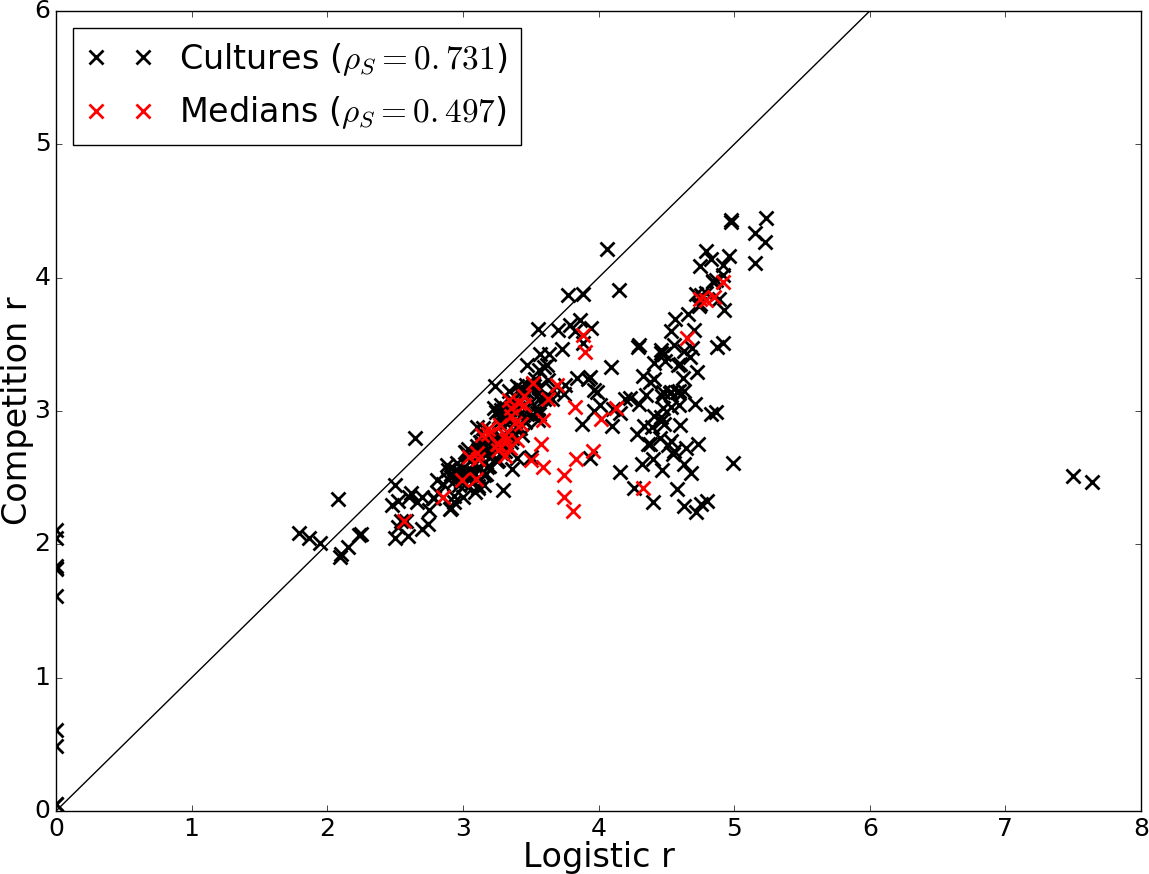
\includegraphics[width=\linewidth]{final/r_correlations_median_spearmans_trimmed_2}
  \captionof{figure}{\textbf{Correlation between logistic and
      competition model r for P15}. Correlations are between estimates
    for each culture (black) and between median estimates (six
    repeats) for each deletion (red). Spearman's rank correlation
    coefficient, \(\rho_{s}\), is displayed for each distribution. The
    line y = x is also plotted.}
  \label{fig:P15_correlations}
\end{Figure}

\subsubsection{Comparison of fitness rankings}

I compared between models the ranking of strains by median fitness
(Figure~\ref{fig:comp_vs_log_ranking}). Rankings of competition model
\(b\), \(r\), and \(MDR\) are equivalent (see
Section~\ref{sec:parameter_conversion}), so I compared \(b\) directly
with logistic model \(r\) and \(MDR\).
% In Figure~\ref{fig:comp_vs_log_ranking}, I compare deletions on P15
% ranked by competition model \(b\), logistic model \(r\), and
% logistic model \(MDR\). The fittest deletions are at the top. For
% each fitness measure, I took the median estimate from repeats of
% each deletion. I used the QFA R package to infer logistic model
% \(r\) and \(MDR\), and used \(b\) from the best fit of the
% competition model (Section~\ref{sec:P15_fit}). Competition model
% \(b\), \(r\), and \(MDR\) rank are equivalent (see
% Section~\ref{sec:parameter_conversion}) so it is not necessary to
% convert \(b\) to compare rankings.
The logistic rankings agree in the order of all but two deletions:
\textit{rad50\(\Delta\)} and \textit{est1\(\Delta\)}. These deletions
each have explained outliers with unrealistically high \(r\) and low
\(K\) (Section~\ref{sec:correlation}). This appears to have been
corrected for when \(MDR\) was calculated (\ref{eq:MDR_MDP}a), and
\(MDR\) rank agrees much better with competition model. Spearman's Rho
is therefore higher between competition \(b\) and logistic \(MDR\)
(0.635) than between competition \(b\) and logistic \(r\)
(0.497). Between models, there is good agreement in extreme positions,
but middle positions are almost inverted. The positions of the neutral
deletion, \textit{his3\(\Delta\)} (bold), disagree by 13 places.

\graphicspath{{images/rank/}}
\begin{Figure}
  \centering
  \includegraphics[width=\linewidth]{final/median_ranks_comp_b_log_r_MDR}
  \captionof{figure}{\textbf{Comparison of competition and logistic
      fitness rankings for P15.} Deletions, each with six repeats, are
    ranked according to median fitness, with the fittest strain at the
    top. Spearman's Rho is 0.497 between competition \(b\) and
    logistic \(r\), and 0.635 between competition \(b\) and logistic
    \(MDR\). \textit{his3\(\Delta\)} (bold) is a neutral deletion with
    14 repeats.}
  \label{fig:comp_vs_log_ranking}
\end{Figure}


% \graphicspath{{images/rank/}}
% \begin{Figure}
%   \centering
%   \includegraphics[width=\linewidth]{final/comp_b_log_r_trimmed}
%   \captionof{figure}{\textbf{Comparison of \(\bm{r}\) ranking for fits
%       of the competition and logistic model to P15.} Fitnesses of
%     genetic strains are ranked most to least fit from top to
%     bottom. Competition model \(r\) was converted from \(b\), \(N_0\),
%     and \(C_0\) from the best competition model estimate. Logistic
%     \(r\) and \(MDR\) were taken from logistic model fits using the
%     QFA R package which makes heuristic checks for slow growing
%     cultures.}
%   \label{fig:comp_vs_log_ranking2}
% \end{Figure}



% Complicated correlation coefficient table
% \columnbreak
% \begin{center}
%   \captionof{table}{\textbf{Correlation coefficients between logistic
%       and competition model estimates of parameters for P15.} Pearson
%     correlation coefficient \(\rho\) and Spearman rank correlation
%     coefficient \(r_{s}\) are shown. Correlation coefficients compare
%     between logistic and competition model estimates for both \(r\)
%     and \(MDR\). Correlations are shown between estimates for each
%     culture and between median and mean estimates for each deletion.}
% \begin{tabular}{ |c|c|c|c|c| } \cline{2-5}
% \multicolumn{1}{c|}{} & \multicolumn{2}{c|}{\(r\)} & \multicolumn{2}{c|}{\(MDR\)}\\ \hline
% \multicolumn{1}{|c|}{Estimates} & \(\rho\) & \(r_{s}\) & \(\rho\) & \(r_{s}\)\\ \hline
% Culture & 0.712 & 0.731 & 0.752 & 0.754\\
% Median & 0.708 & 0.497 & 0.791 & 0.635\\
% Mean   & 0.763 & 0.594 & 0.885 & 0.732\\ \hline
% \end{tabular}
% \end{center}

% Just a fit of a zone
% \end{multicols}
% \graphicspath{{images/comp_fit/}}
% \begin{Figure}
%   \centering
%   \includegraphics[width=\linewidth]{final/P15_guess_and_fit_r5_c18}
%   \captionof{figure}{\textbf{A zone of a fit of the competition model
%       to P15 and initial guess}. The guess was made using the
%     imaginary neighbour model fit to individual cultures. Top-left
%     coordinates from Figure~\ref{fig:comp_fit_plate} (5, 18).}
%   \label{fig:comp_fit_zone_old}
% \end{Figure}
% \begin{multicols}{2}





% Make landscape and take a whole page.
\end{multicols}
\begin{landscape}
\graphicspath{{images/comp_fit/}}
\begin{Figure}
  \centering
  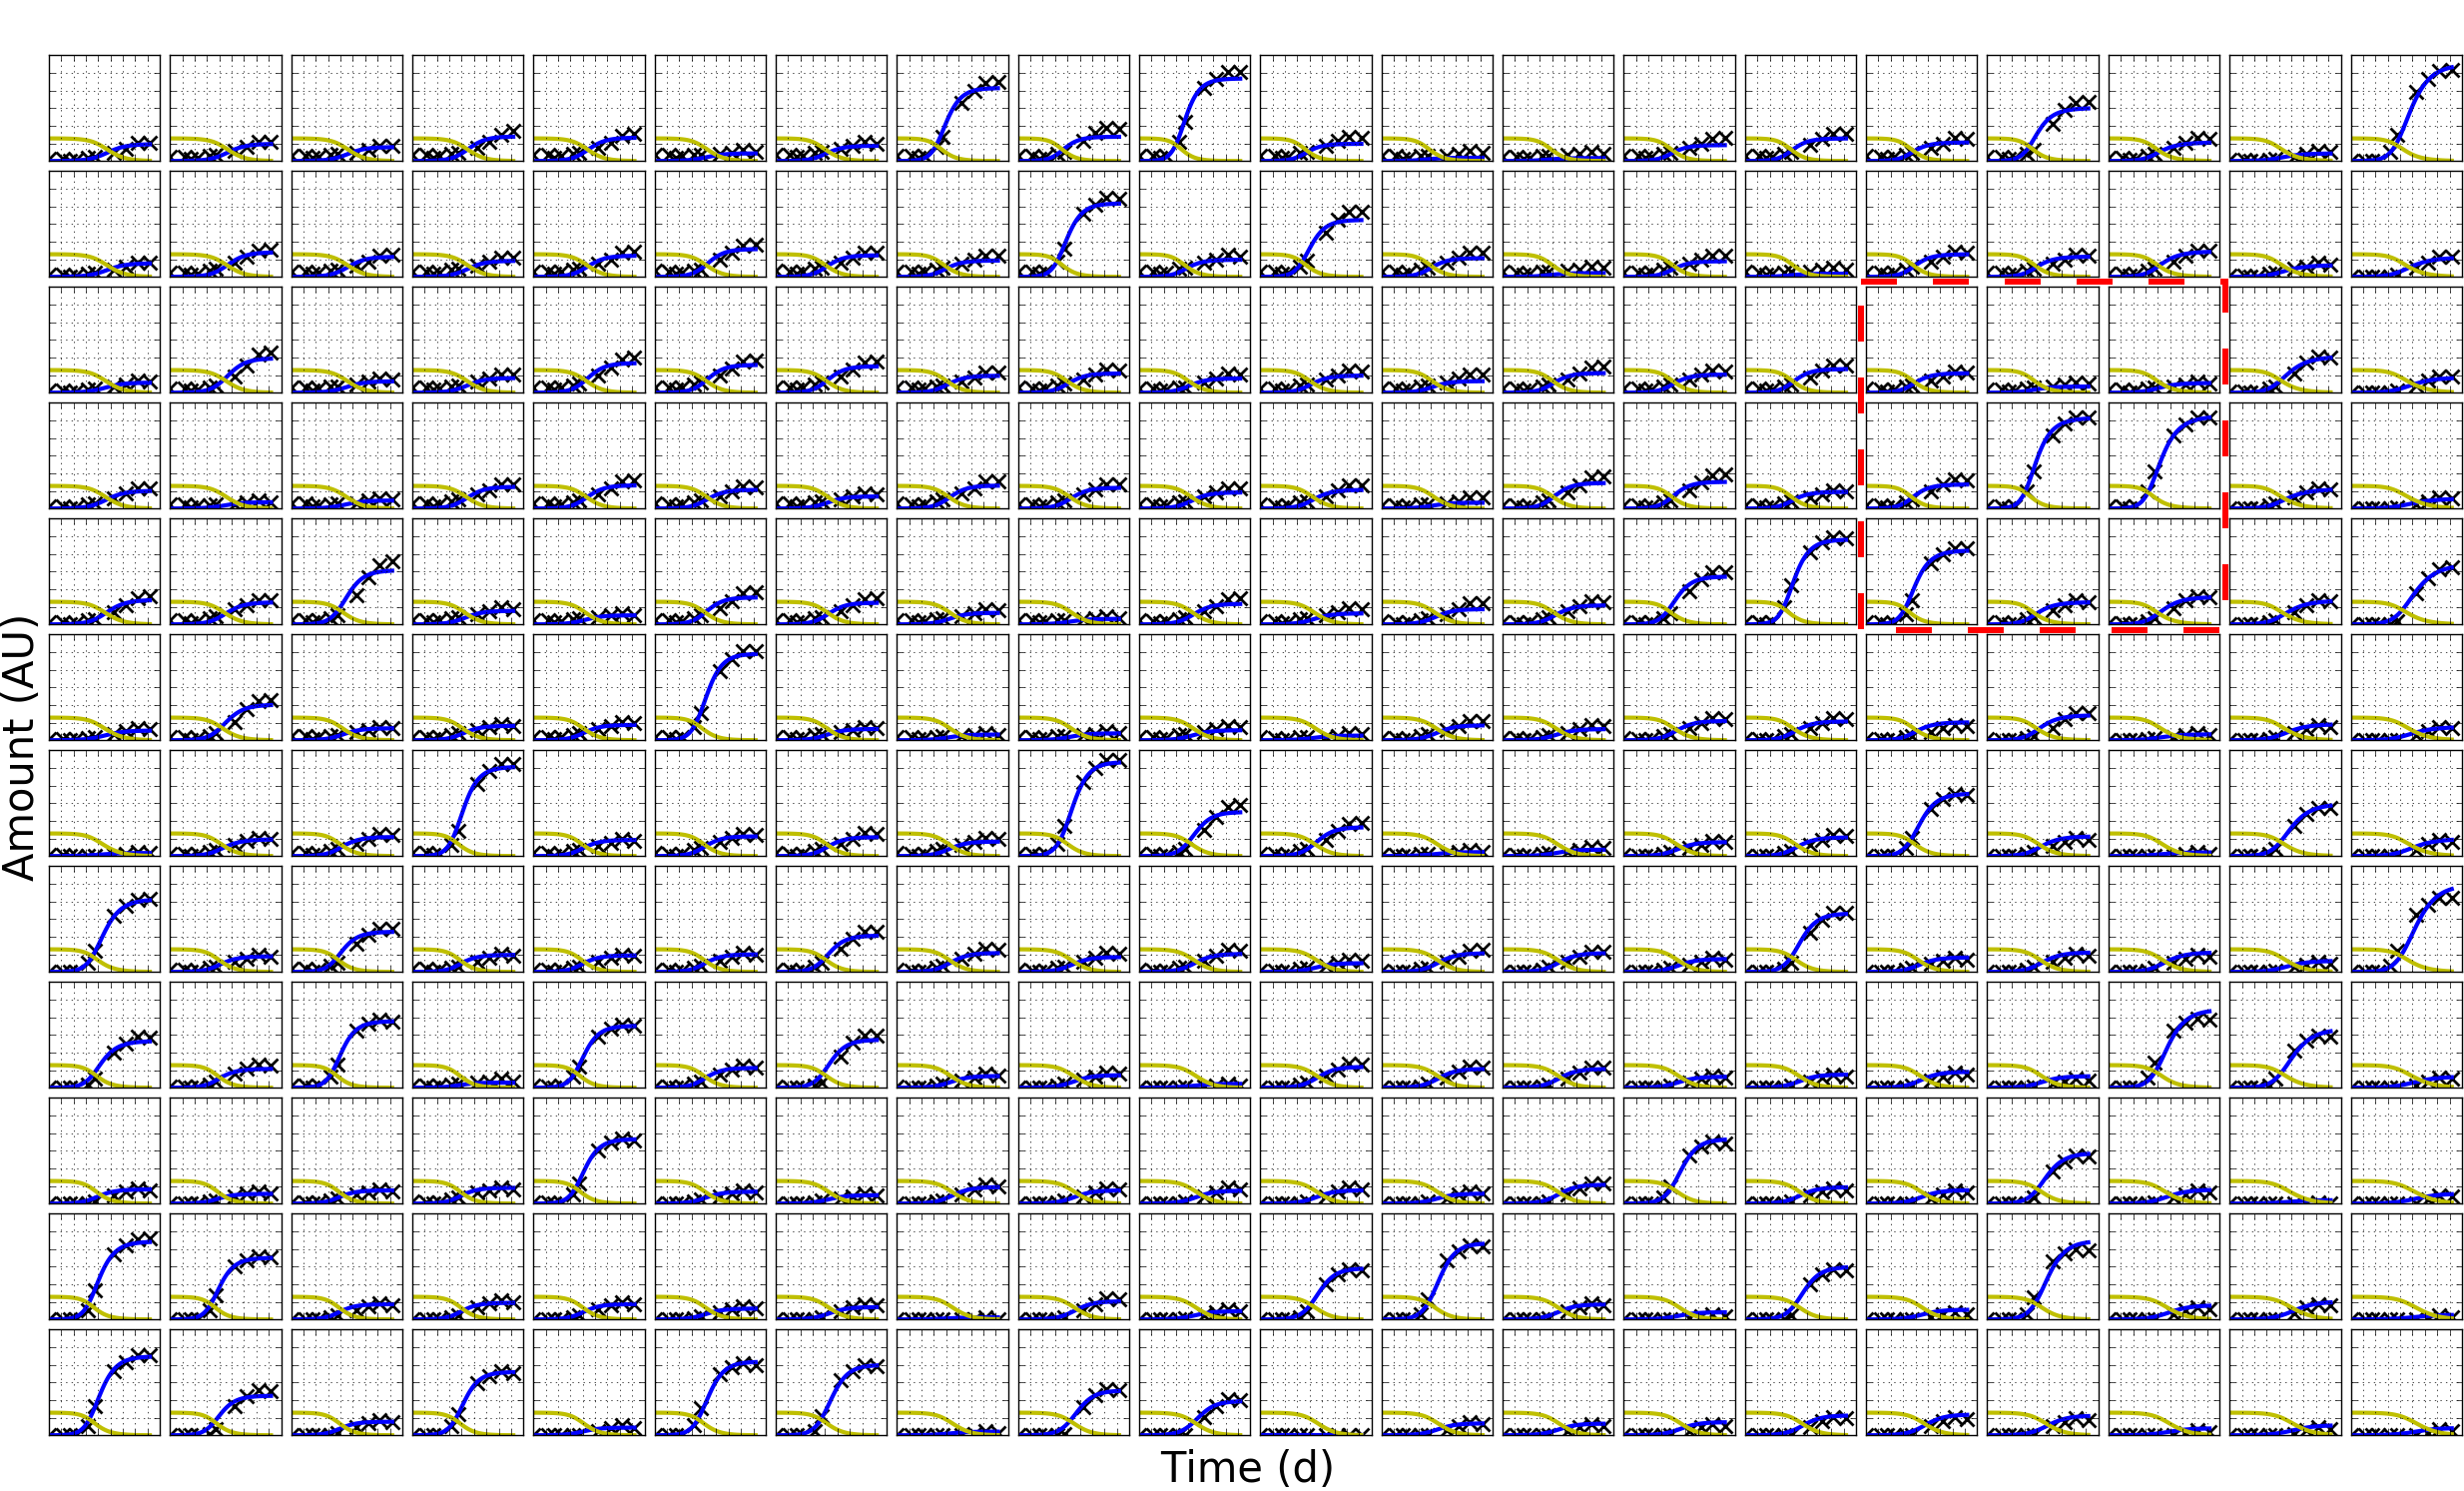
\includegraphics[width=\linewidth]{full_plate/final/P15_12x20_2}
  \captionof{figure}{\textbf{Fit of the competition model to P15.}
    Data is for a 16x24 format plate (P15) with background mutation
    \textit{cdc13-1} incubated at 27\(^{\circ}C\). The plate contains
    6 repeats of 50 genetic strains randomly arranged across the
    internal cultures. Repeats of a single strain are used for all
    edge cultures (removed in the plot). Model output for state
    variable, cell population size (blue curve), is fit to observed
    data (black crosses). Model predictions for unobserved variable
    (nutrient amount) are also plotted (yellow). The outer two rows
    and columns have been removed. See Figure~\ref{fig:P15_zone_fit}
    for a larger plot of the boxed zone.}
  \label{fig:comp_fit_plate}
\end{Figure}
\end{landscape}
\begin{multicols}{2}



\subsubsection{Evaluating the treatment of boundaries}
\label{sec:treatment_of_boundaries}

I had seen that objective function values were large for edge cultures
compared to internal cultures (Table~\ref{tab:P15_obj_fun}). To
evaluate the treatment of boundaries, I also fit the one \(N(0)\)
parameter competition model to P15 using the same method as for the
two \(N(0)\) parameter model (see Section~\ref{sec:P15_fit}). Fits
appear similar in quality for both models
(Figure~\ref{fig:P15_corner}) and average objective function values
for the entire plate are very similar
(Table~\ref{tab:corner}). Objective function values for cultures next
to an edge culture are improved with the two \(N(0)\) model and
internal cultures were better fit overall. Interestingly, fits of the
edge cultures are actually worse in the two \(N(0)\) model. These
cultures are dominated by noise due to reflections from plate walls
which is why they are discarded from final estimates. However, the
edge cultures must be included in the objective function when fitting
the competition model. Despite this deficit, the two \(N(0)\) model
has increased the goodness of fit to internal cultures by collectively
fitting all cultures.


\graphicspath{{images/corners/}}
\begin{Figure}
  \centering
  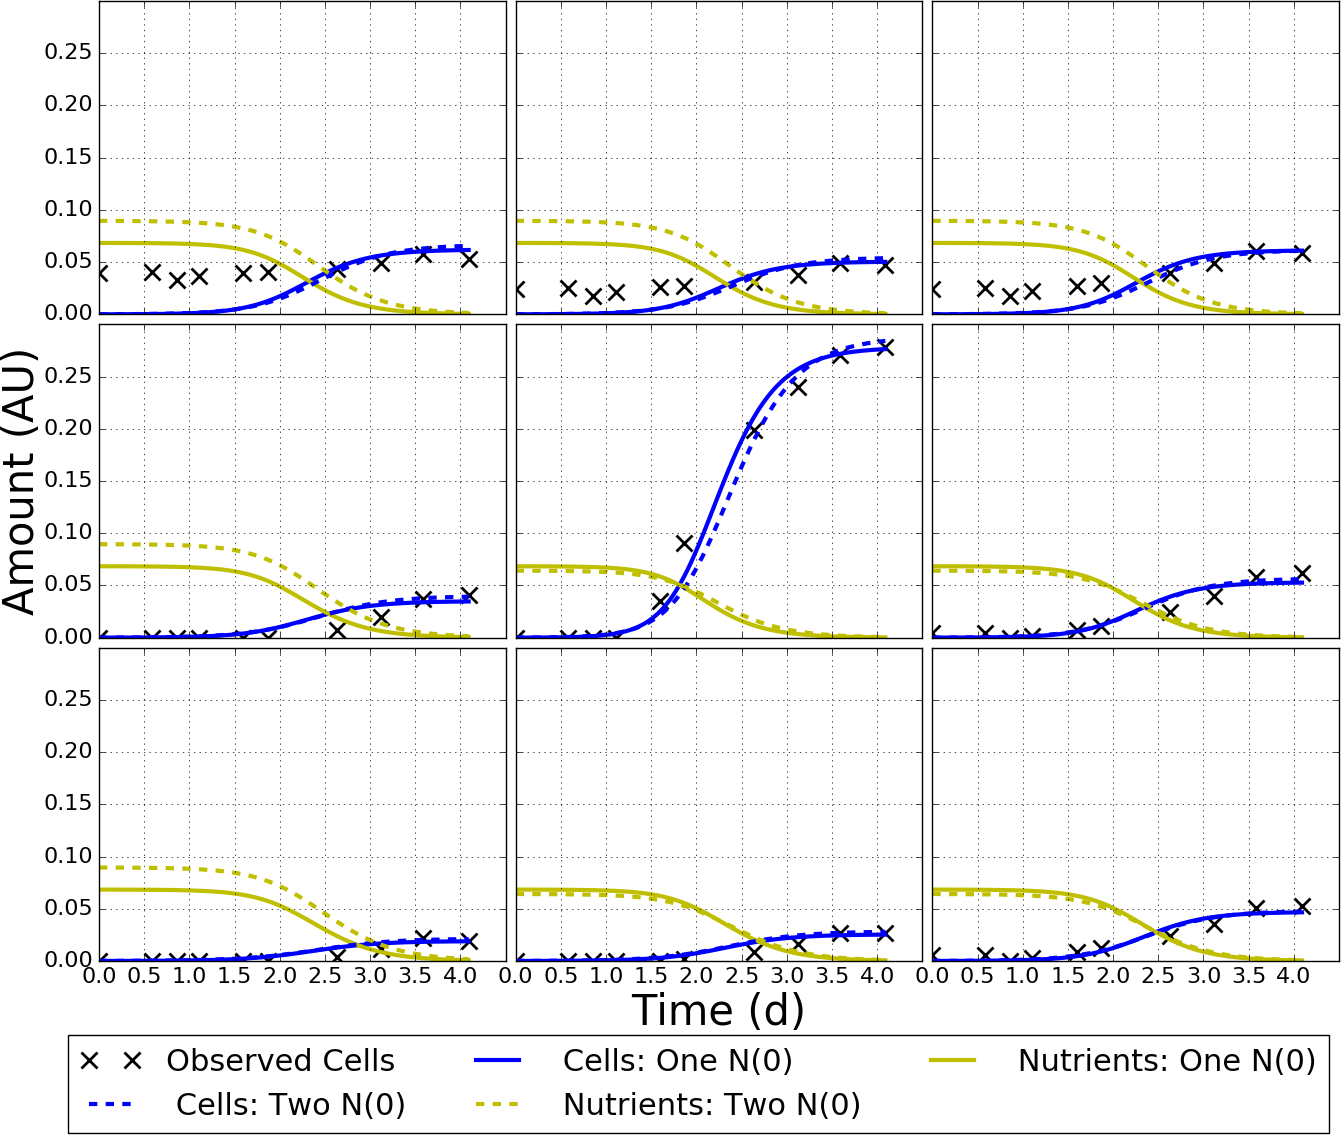
\includegraphics[width=\linewidth]{final/top_left_new_aspect_2}
  \captionof{figure}{\textbf{Treatment of boundary conditions in fits
      of the competition model.} The top left corner of a 16x24 QFA
    plate (P15) fitted with two versions of the competition model: the
    first with a single initial nutrient amount for all cultures, the
    second with a separate initial nutrient amount for edge cultures.}
  \label{fig:P15_corner}
\end{Figure}


\begin{center}
  \captionof{table}{\textbf{Average objective function value for one a
      two \(\bm{N(0)}\) parameter competition models.} Values are for
    the same fits as in Figure~\ref{fig:P15_corner} and have been
    scaled by \(10^{4}\). Averages are for cultures belonging to the
    areas indicated by the column ``Cultures''. ``Next to edge''
    refers to cultures one in from the edge. ``Internal'' refers to
    all cultures but the edge. Lower values are better.}
  \begin{tabular}{l l l}
    \hline
    Cultures     & One \(N(0)\)  & Two \(N(0)\) \\
    \hline
    Edge         & 35.9    & 36.5\\
    Next to edge & 9.54    & 7.98\\
    Internal     & 6.67    & 6.30\\
    All          & 12.4    & 12.2\\
    \hline
  \end{tabular}
  \label{tab:corner}
\end{center}

% \subsection{\thesubsection~Agreement of b rankings}

%   text Some text Some text Some text Some text Some text Some text
%   Some text Some text Some text Some text.
% \graphicspath{{images/rank/}}
% \begin{Figure}
%   \centering
%   \includegraphics[width=\linewidth]{top_two_comp_p15_correlations_trimmed}
%   \captionof{figure}{\textbf{Comparison of \(\bm{b}\) ranking for the
%       best five competition model fits to P15.} Ranking is calculated
%     from the mean \(b\) estimate from the six repeats or each strain.}
%   \label{fig:comp_b_ranking}
% \end{Figure}


\subsubsection{Precision of fitness estimates}
\label{sec:cross_plate_validation}

% Use repeats on plate 15 (6 per deletion) more (14) for HIS3 to
% calculate coefficient of variation (COV) of estimated r or MDR.

In Figure~\ref{fig:COV}, I compare coefficients of variation (COVs)
for competition model estimates of \(b\) and logistic model estimates
of \(r\) between repeats of each deletion on P15. I chose to compare
\(b\) and \(r\), rather than \(b\) and \(MDR\), because both
parameters are growth constants in the competition and logistic models
respectively. Regardless, COVs for \(MDR\) (not shown) are very
similar to COVs for \(r\). The precision of fitness estimates is of
interest both as a test of the model and because it affects the power
to infer genetic interactions. If we assume that biological variation
in fitness between repeats of the same strain is small, then the
better model should estimate the fitness of strains more precisely,
regardless of where repeats are grown on the plate.

Deletions in Figure~\ref{fig:COV} are arranged from left to right
according to competition model \(b\) ranking, with the fastest growing
deletion on the left. The competition model has a smaller COV for 36
out of 50 deletions. However, the logistic model has a smaller COV for
the 11 fastest growers (according to \(b\) ranking). Comparing with
Figure~\ref{fig:P15_correlations}, median values for these deletions
(red) appear in the upper right of both groups of cultures (black),
not in the gap inbetween. \(b\) COV tends to be smaller than \(r\) COV
at smaller values of \(b\), where repeats are likely to divided
between the groups (as indicated by the positions of medians inbetween
groups). The slowest growers tend to have greater COV for both models,
which is likely due to the greater effect of noise on cell density
estimates in repeats of these deletions.

\end{multicols}
\graphicspath{{images/COV/}}
\begin{Figure}
  \centering
  \includegraphics[width=\linewidth]{final/comp_b_log_r_median_rank_his3_bold}
  \captionof{figure}{\textbf{Coefficients of variation (COVs) for
      growth estimates from P15.} COVs are shown for competition model
    \(b\) and logistic model \(r\) estimates for repeats of each
    deletion. COVs of competition model \(b\) and \(r\) are equivalent
    (see Section~\ref{sec:parameter_conversion}). Deletions are
    ordered left to right along the horizontal axis from highest to
    lowest competition model \(b\) ranking. Logistic fits used the QFA
    R package.}
  \label{fig:COV}
\end{Figure}
\begin{multicols}{2}


\end{multicols}
\graphicspath{{images/stripes/}}
\begin{Figure}
  \centering
  \includegraphics[width=\linewidth]{final/validation_r9_c10_no_nutrients}
  \captionof{figure}{\textbf{Calibration and validation of the
      competition model.} I fit the competition model to the 16x24
    format ``Stripes'' and ``Filled'' plates
    (Section~\ref{sec:stripes_description}). The plot shows cell
    measurements and estimates for both plates for a 3x3 section with
    top left coordinates (R9, C10). I took the parameters estimates
    for the ``Filled'' plate (calibration) and set growth constants,
    \(b_{i}\), to zero for cultures in the empty columns of the
    ``Stripes'' plate. I then simulated using these parameters to
    produce the dashed blue curve (validation). If the model corrects
    for differences in growth between these experimental designs
    perfectly, the dashed blue curves should resemble the ``Stripes''
    data (blue crosses) in columns one and three. The logistic model
    would predict no change in growth between plates.}
  \label{fig:stripes_validation}
\end{Figure}
\begin{multicols}{2}

\subsection{Cross-plate validation}
\label{sec:cross_plate_val_results}

I used the Stripes and Filled plates experiment
(Figure~\ref{fig:stripes_images}) to conduct cross plate calibration
and validation of the competition model. As for P15
(Section~\ref{sec:P15_fit}), I ran multiple fits of the competition
model for each plate. Due to the greater number of timepoints in the
data, I fit to cell densities at 15 evenly spaced timepoints taken
from a spline of the observed data to increase the speed of fitting
(see Section~\ref{sec:solving_comp}). I used a greater range of
\(C(0)\) guesses than for P15: 10 values ranging from
\(N(0)\times\)10\(^{-7}\) to \(N(0)\times\)10\(^{-1}\) in logspace. I
made this decision due to the higher inoculum densities used in these
plates and as a result of discussion with Herrmann and Lawless, who
had suggested, based on recent work, that heterogeneity exists within
individual cultures such that only a small number of cell lines
contribute significantly to final populations. Again, each fit used
the imaginary neighbour model to make initial guesses of \(b_{i}\)
with 14 different initial \(b\) guesses for each \(C(0)\) guess
(Section~\ref{sec:guessing_b}). This made a total of 140 fits to each
plate. I guessed other parameters as described in
Section~\ref{sec:initial_guess} and used separate parameters for the
initial amount of nutrients in edge and internal cultures.

The experiment, described in detail in
Section~\ref{sec:stripes_description}, is designed to test for
competition effects.
% Already mentioned - just refer to methods is needs be: I received
% data from E. Holstein (April 2016) in personal communications.
The strains in the Stripes plate (Figure~\ref{fig:stripes_images}a)
are inoculated in the same positions on the Filled plate
(Figure~\ref{fig:stripes_images}b). I took the competition model
parameter estimates for the Filled plate and simulated the Stripes
plate by setting \(b\) to zero for locations in the gaps on this
plate. I compared the resulting timecourses with the Stripes cell
observations (Figure~\ref{fig:stripes_validation}). If the competition
model corrects for differences between the plates perfectly, then the
simulated timecourses (blue dashes) should fit closely to the Stripes
data (blue crosses). I found that the competition model overcorrects
for competition; simulated cell densities are higher than observations
across the plate. In contrast, the logistic model makes no adjustment
between plates and would underestimate observed cell densities by a
similar amount. There are some issues with the data set. For instance,
the top right culture in Figure~\ref{fig:stripes_validation} does not
grow and may have been inoculated with dead cells. However, these
mistakes are unlikely to have caused the systematic overcorrection
that is observed. Data for empty cultures on the Stripes plate (blue
crosses, middle column) is just noise and I excluded these timecourses
from the objective function when fitting.

\begin{center}
  \captionof{table}{\textbf{Estimated parameter values for the best
      two competition model fits to P15.} Spearman's rank correlation
    coefficient (\(\rho_{s}\)) for \(b\) estimates of the cultures in
    common is 0.787.}
  \begin{tabular}{l l l l l l}
    \hline
    Plate     & \(C(0)\)                   & \(N_{I}(0)\) & \(N_{E}(0)\) & \(k\) & \(b\) (mean)\\
    \hline
    Stripes   & 8.3\(\times\)10\(^{-3}\)   & 0.085      & 0.096       & 1.9  & 39.5\\
    Filled    & 6.2\(\times\)10\(^{-3}\)   & 0.116      & 0.183       & 4.8  & 27.9\\
    \hline
  \end{tabular}
  \label{tab:Stripes_and_Filled_params}
\end{center}

The inferred parameters for the best competition model fits to both
plates are shown in Table~\ref{tab:Stripes_and_Filled_params}. Both
plates used the same inoculum density and formula of agar so I did not
expect plate level parameters to vary between plates. However, there
is significant disagreement in all parameters, indicating that the
competition model is not working correctly. There was also more
disagreement in the top fits for each plate than was the case for P15,
which used a lower inoculum density. Estimates for the five best fits
to the Filled plate (Table~\ref{tab:Stripes_and_Filled_params}) are
only consistent for initial nutrient densities. Despite this, they all
overestimated growth when used to simulate the Stripes
plate. Disagreement between the best estimates was worse still for the
Stripes plate (not shown).

\begin{center}
  \captionof{table}{\textbf{Estimated parameter values for the best
      five competition model fits to the Filled plate.} Estimates are
    ordered by objective function values (Obj.) of the fits where
    lower values are better. The column MAD \(b\) is the mean absolute
    deviation of growth constants \(b_{i}\) with those of the best fit
    (row one). Mean \(b\) for the best fit was 27.9. Spearman's
    \(\rho_{S}\) > 0.96 for all correlations of these fits.}
  \begin{tabular}{l l l l l l}
    \hline
    Obj.  & \(C(0)\)                  & \(N_{I}(0)\) & \(N_{E}(0)\) & \(k\) & MAD \(b\)\\
    \hline
    0.76  & 6.2\(\times\)10\(^{-3}\)   & 0.116       & 0.183    & 4.8  & -    \\
    0.85  & 5.6\(\times\)10\(^{-3}\)   & 0.119       & 0.175    & 3.1  & 0.77 \\
    0.88  & 5.0\(\times\)10\(^{-3}\)   & 0.119       & 0.175    & 2.9  & 1.65 \\
    0.93  & 15.4\(\times\)10\(^{-3}\)  & 0.114       & 0.171    & 4.7  & 11.1 \\
    0.97  & 3.2\(\times\)10\(^{-3}\)   & 0.118       & 0.179    & 3.8  & 7.80 \\
    \hline
  \end{tabular}
  \label{tab:Filled_best_fits}
\end{center}
% \begin{center}
%   \captionof{table}{\textbf{Parameter bounds.} Used for fitting the
%     competition model to P15 and the Stripes and Filled plates. Bounds
%     on \(N(0)\) were applied to both \(N^{I}(0)\) and
%     \(N^{E}(0)\) for internal and edge cultures. ``guess'' refers
%     to the initial guess (see Section~\ref{sec:initial_guess}).}
%   \begin{tabular}{| c | c c |}
%     \hline
%     Parameter        & Stripes  & Filled \\
%     \hline
%     Spearman's \(C(0)\)     & guess x \(10^{-3}\)  & guess x \(10^{3}\)\\
%     \(N(0)\)     & guess / \(2\)  & guess x \(2\)\\
%     % \(N^{I}(0)\) \& \(N^{E}(0)\) & guess / \(2\)  & guess x \(2\)\\\\
%     \(k\)        & 0.0    & 10.0\\
%     % \(b\) (all cultures)           & 0.0    & \(\infty\) \\
%     \(b\)           & 0.0    & None \\
%     \hline
%   \end{tabular}
%   \label{tab:stipes_agreements}
% \end{center}
% \graphicspath{{images/stripes/}}
% \begin{Figure}
%   \centering
%   \includegraphics[width=\linewidth]{final/r_correlations_between_plates_A}
%   \includegraphics[width=\linewidth]{final/r_correlations_between_models_B_colours_2}
%   \captionof{figure}{\textbf{Correlation of r estimates for
%       ``Stripes'' and ``Filled'' plates.}~A) Correlation of r
%     estimates between plates for logistic and competition
%     models. B) Correlation of r estimates between logistic and
%     competition models for both plates.  I fit the competition model
%     and independent model to the ``Stripes'' and ``Filled'' plates in
%     Figure~\ref{fig:stripes_images}. I converted competition model b
%     to logistic model r. I only used data for cultures that were
%     common between the two plates common and removed edge
%     cultures. Pearson correlation coefficients, \(\rho\), are shown
%     in the legends. The line \(y=x\) is also plotted.}
%   \label{fig:r_correlations_v2}
% \end{Figure}
% \graphicspath{{images/stripes/correlations/}}
% \begin{Figure}
%   \centering
%   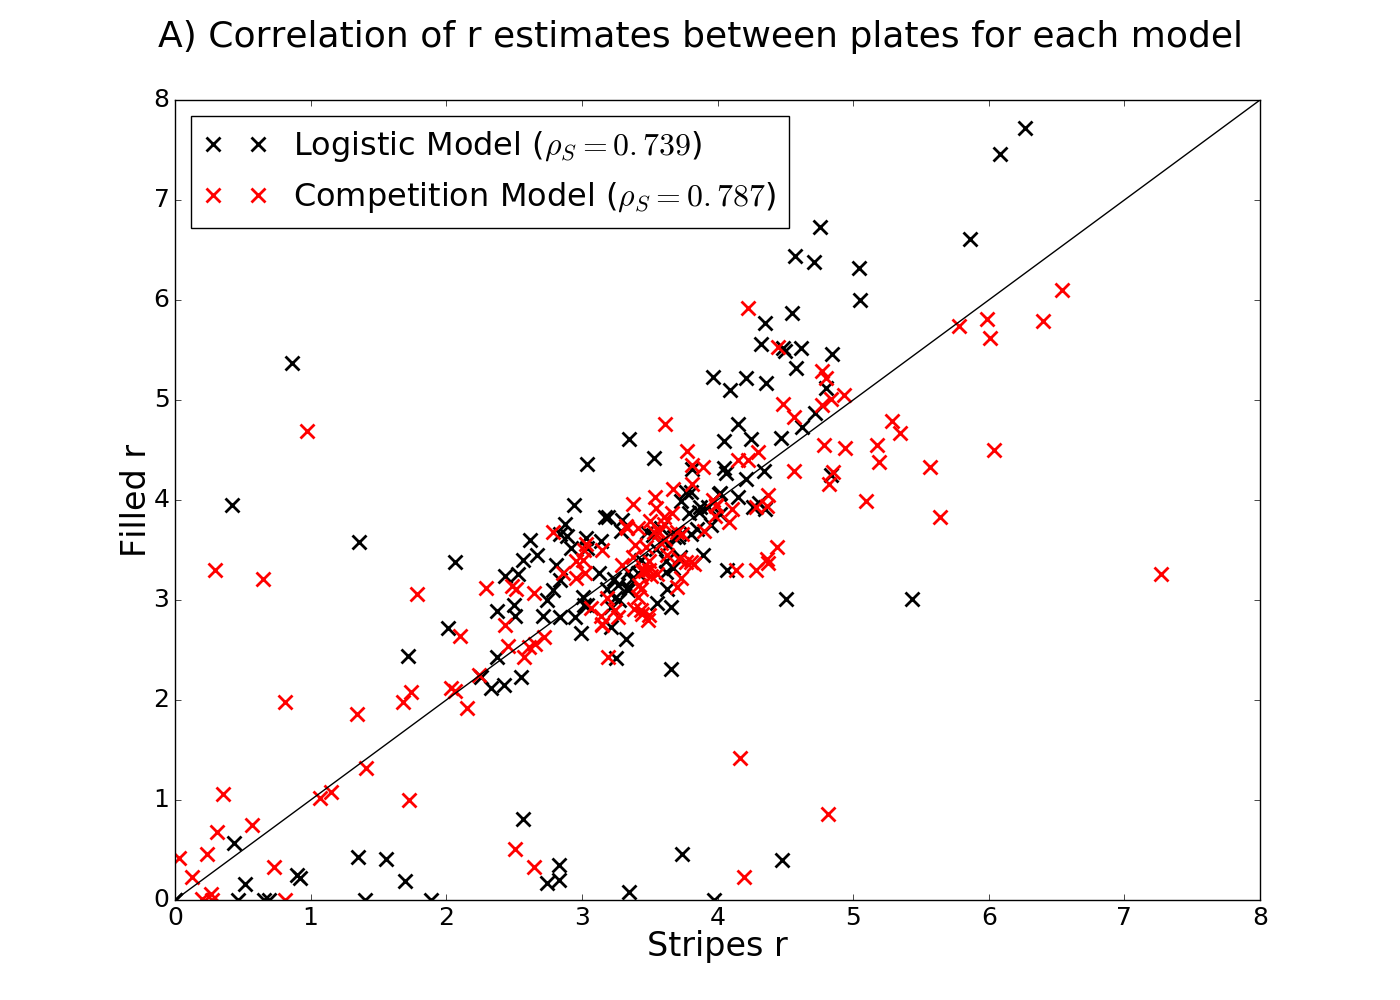
\includegraphics[width=\linewidth]{final/r_correlations_between_plates}
%   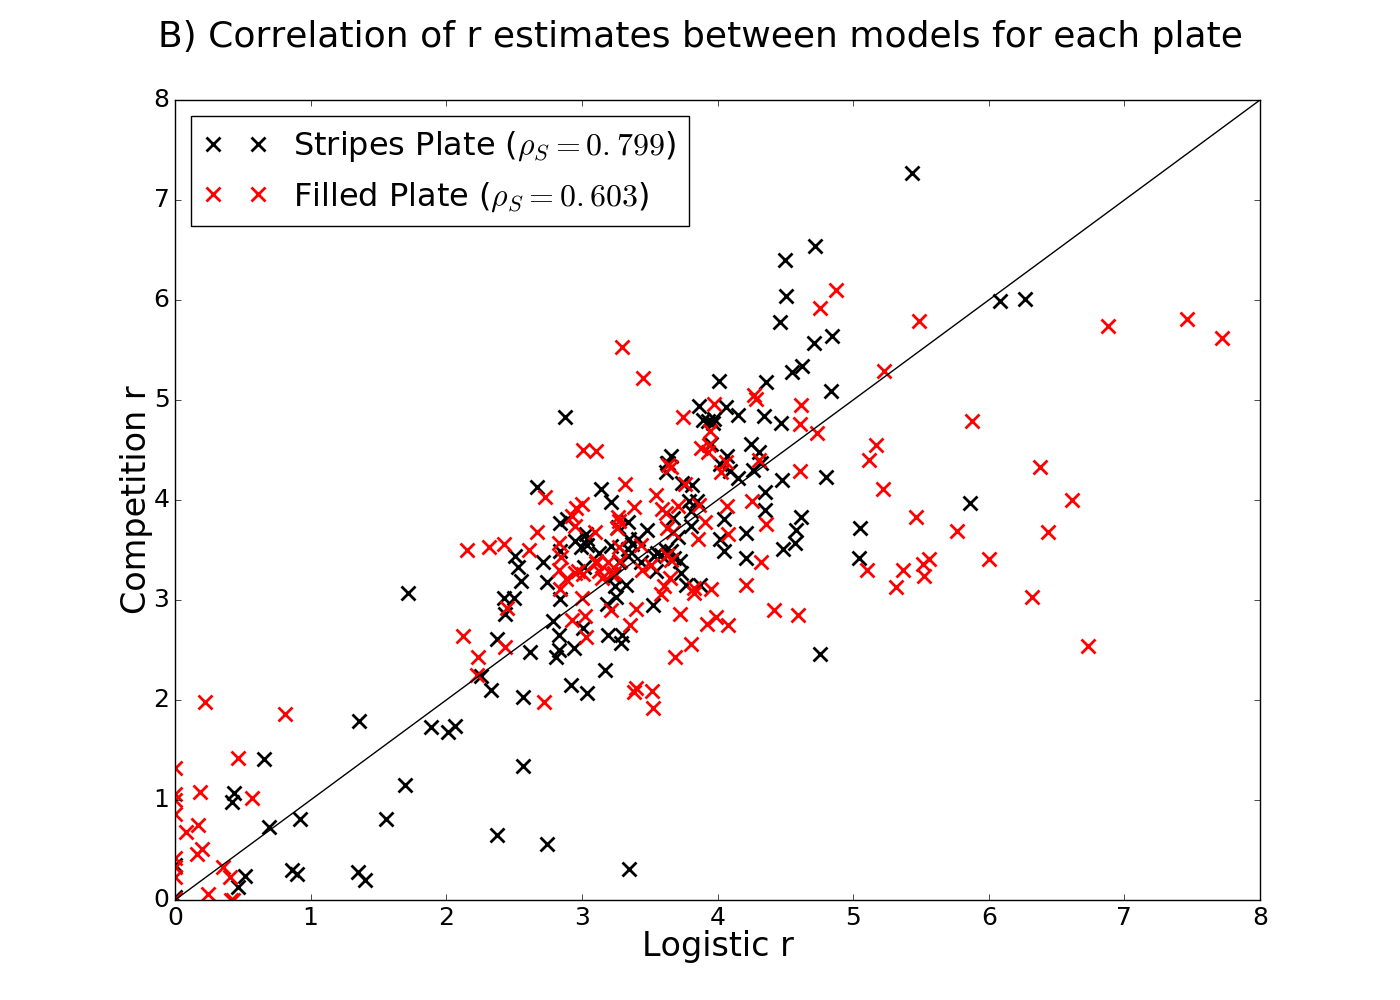
\includegraphics[width=\linewidth]{final/r_correlations_between_models}
%   \captionof{figure}{\textbf{Correlation of r estimates for
%       ``Stripes'' and ``Filled'' plates.}~I fit the competition model
%     and independent model to the ``Stripes'' and ``Filled'' plates in
%     Figure~\ref{fig:stripes_images}. I converted competition model b
%     to logistic model r. I only used data for cultures that were
%     common between the two plates common and removed edge
%     cultures. Pearson correlation coefficients, \(\rho\), are shown in
%     the legends. The line \(y=x\) is also plotted.}
%   \label{fig:r_correlations}
% \end{Figure}

\subsection{Towards a genetic algorithm}

% %\end{multicols}
% \graphicspath{{images/genetic_algorithm/}}
% \begin{Figure}
%   \centering
%   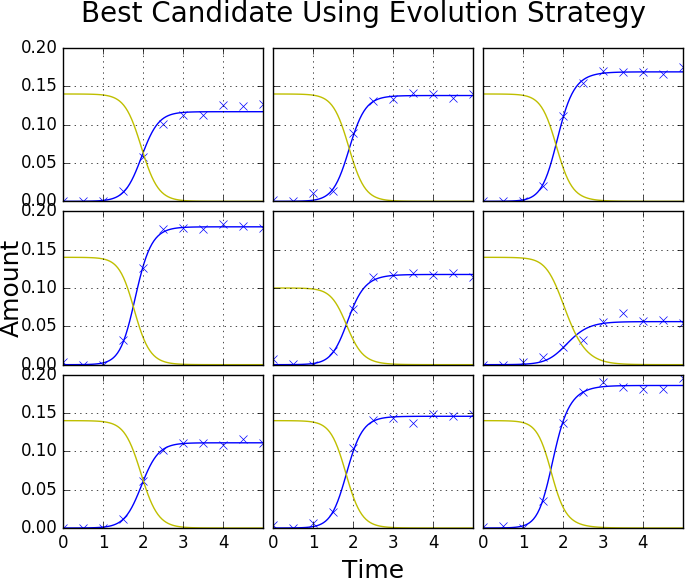
\includegraphics[width=\linewidth]{final/ga_fit_to_sim_true_plate_lvl_trimmed}
%   \captionof{figure}{Genetic algorithm fit to a 3x3 simulation. MIGHT
%     TAKE A LITTLE BIT OF WORK TO REPRODUCE AND COULD USE PARAMETERS
%     FROM THE BEST P15 FIT RATHER THAN JUST PICKING/RANDOMIZING. NEED
%     TO CHECK THAT PLATE LEVEL PARAMETERS WERE ALSO EVOLVED.}
%   \label{fig:3x3_genetic_algorithm_comp_fit_fixed_plate_level}
% \end{Figure}
% %\begin{multicols}{2}
%\end{multicols}
\graphicspath{{images/genetic_algorithm/}}
\begin{Figure}
  \centering
  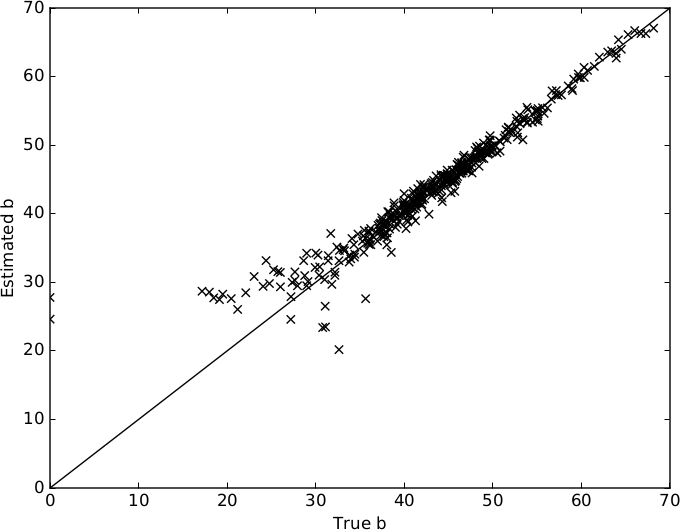
\includegraphics[width=\linewidth]{final/est_b_vs_true_b}
  \captionof{figure}{\textbf{Recovery of true \(b\) values from a
      gradient fit to simulated date using fixed plate level
      parameters.} I simulated timecourses from the best five
    competition model fits to p15, added a small amount of noise, and
    used a gradient method to recover b given the true plate level
    parameters. This plot shows the worst case from the five sets of
    values.}
  \label{fig:comp_fit_fixed_plate_level}
\end{Figure}

% Due to the disagreement between competition model estimates for the
% same plates, I was motivated to explore alternative strategies for
% fitting that might return global minima.
To test the viability of using a genetic algorithm to evolve
plate-level parameter candidates to be evaluated using a gradient
method, I took parameter estimates from the five best fits for P15,
and simulated full plate timecoureses of cell observations with 15
timepoints. I added a small amount of random noise to each timecourse
to replicate real data. I then fixed the plate level parameters to the
true values and fit the competition model just for
\(b_{i}\). \(b_{i}\) were recovered well even in the worst instance
(Figure~\ref{fig:comp_fit_fixed_plate_level}). Estimates are worse for
slow growing cultures which are more affected by noise.


% (Currently only have comp obj funs using different cultures (Stripes
% obj fun 0.66) (Filled obj fun 0.76).)


%\begin{multicols}{2}

%%% Local Variables:
%%% mode: latex
%%% TeX-master: "report"
%%% End:
